\documentclass{language-supplements}

% commented out these packages for submission to Language
%\usepackage[margin=1in,top=1in,bottom=1in]{geometry}

\usepackage{tikz}
\usepackage{mathtools}
\usepackage{longtable}
\usepackage{enumitem}
\usepackage[hidelinks]{hyperref}
%\usepackage[dvips]{graphics}
%\usepackage[table]{xcolor}
%\usepackage{amssymb}
\usepackage{float}
%\usepackage{subfig}
\usepackage{booktabs}
\usepackage{subcaption}

\usepackage[normalem]{ulem}

\usepackage{multicol}
\usepackage{times}
\usepackage{amsfonts}
%\usepackage{natbib}
\usepackage{gb4e}
\usepackage[all]{xy}
\usepackage{rotating}
\usepackage{tipa}
\usepackage{multirow}
\usepackage{authblk}
\usepackage{url}
\usepackage{pdflscape}
\usepackage{rotating}
\usepackage{adjustbox}
\usepackage{array}


\def\bad{{\leavevmode\llap{*}}}
\def\marginal{{\leavevmode\llap{?}}}
\def\verymarginal{{\leavevmode\llap{??}}}
\def\swmarginal{{\leavevmode\llap{4}}}
\def\infelic{{\leavevmode\llap{\#}}}

\definecolor{airforceblue}{rgb}{0.36, 0.54, 0.66}
%\definecolor{gray}{rgb}{0.36, 0.54, 0.66}

\definecolor{Pink}{RGB}{240,0,120}
\newcommand{\red}[1]{\textcolor{Pink}{#1}}
\newcommand{\jd}[1]{\textbf{\textcolor{Pink}{[jd: #1]}}}

\newcommand{\dashrule}[1][black]{%
  \color{#1}\rule[\dimexpr.5ex-.2pt]{4pt}{.4pt}\xleaders\hbox{\rule{4pt}{0pt}\rule[\dimexpr.5ex-.2pt]{4pt}{.4pt}}\hfill\kern0pt%
}

\setlength{\parindent}{.3in}
\setlength{\parskip}{0ex}

\newcommand{\yi}{\'{\symbol{16}}}
\newcommand{\nasi}{\~{\symbol{16}}}
\newcommand{\hina}{h\nasi na}
\newcommand{\ina}{\nasi na}

\newcommand{\foc}{$_{\mbox{\small F}}$}

\hyphenation{par-ti-ci-pa-tion}

\setlength{\bibhang}{0.5in}
\setlength{\bibsep}{0mm}
\bibpunct[:]{(}{)}{,}{a}{}{,}

\newcommand{\6}{\mbox{$[\hspace*{-.6mm}[$}} 
\newcommand{\9}{\mbox{$]\hspace*{-.6mm}]$}}
\newcommand{\sem}[2]{\6#1\9$^{#2}$}
\renewcommand{\ni}{\~{\i}}

\newcommand{\citepos}[1]{\citeauthor{#1}'s \citeyear{#1}}
\newcommand{\citeposs}[1]{\citeauthor{#1}'s}
\newcommand{\citetpos}[1]{\citeauthor{#1}'s (\citeyear{#1}}

\newcolumntype{R}[2]{%
    >{\adjustbox{angle=#1,lap=\width-(#2)}\bgroup}%
    l%
    <{\egroup}%
}
\newcommand*\rot{\multicolumn{1}{R{90}{0em}}}% no optional argument here, please!


\title{Supplementary materials for ``Are there factive predicates? An empirical investigation"}

\author{Judith Degen\\Department of Linguistics\\Stanford University\\
450 Serra Mall \\
Stanford, CA 94305, USA\\ {\tt jdegen@stanford.edu}
\and
 Judith Tonhauser\\Department of Linguistics\\
University of Stuttgart \\
Keplerstr. 17 \\ 
70174 Stuttgart, Germany \\ {\tt judith.tonhauser@ling.uni-stuttgart.de}}

\date{}

\newcommand{\jt}[1]{\textbf{\color{blue}JT: #1}}

\begin{document}

\maketitle

\appendix

\setcounter{page}{1}
%\renewcommand{\thetable}{A\arabic{table}}

\setcounter{table}{0}
\renewcommand{\thetable}{A\arabic{table}}

\setcounter{figure}{0}
\renewcommand{\thefigure}{A\arabic{figure}}

%\section{Citations}
%
%That both properties are ascribed to presuppositions, including the CC of factive predicates, can be seen from the following quotes:
%
%\begin{itemize}[topsep=0pt,itemsep=-3pt,leftmargin=12pt]
%
%\item \citealt[66f.]{beaver01}: \citet[119-123]{gazdar79a} `describes the inferences associated with factive verbs, definite descriptions, aspectual verbs, and clefts as being indefeasible in simple affirmative sentences', that is, `entailments'.
%
%\item \citealt[355]{ccmg90}: `A sentence can both entail and presuppose another sentence [...]. Thus, [{\em Joan realizes that syntax deals with sentence structure}] both entails and presupposes [{\em Syntax deals with sentence struture}].'
%
%\item \citealt[345]{vds92}: `Note that [global accommodation, that is, projectivity, JT\&JD] is what we would expect given the intuitive notion of presupposition as information taken for granted and note also that this explains the intuition that presuppositions [...] are entailed by their matrix sentence.'
%
%\item \citealt[3]{abbott06}: `we will need to be careful to distinguish entailments that are presupposed from what I will call `ordinary, simple entailments', which are not also presuppositions.'
%
%\item \citealt[139]{schlenker10}: `we obtain the pattern of inference which is characteristic of presuppositions: an entailment of the positive sentence is preserved under negation and in questions'
%
%
%\item \citealt[77]{anand-hacquard2014}: `we will adopt the pragmatic view of presupposition triggering, according to which presuppositions are lexical entailments that are backgrounded based on pragmatic principles'
%
%\item {\bf \citealt[fn.7]{spector-egre2015}: Assuming that any presupposition of a sentence is also an entailment of this sentence, it follows that a predicate that is factive with respect to its declarative complement is always also veridical with respect to its declarative complement.}
%
%\end{itemize}

\section{20 complement clauses}\label{a-clauses}

The following clauses realized the complements of the predicates in Exps.~1, 2, and 3: 

\begin{enumerate}[leftmargin=3ex,itemsep=-2pt]

\begin{multicols}{2}

\item Mary is pregnant.
\item Josie went on vacation to France.
\item Emma studied on Saturday morning.
\item Olivia sleeps until noon.
\item Sophia got a tattoo.
\item Mia drank 2 cocktails last night.
\item Isabella ate a steak on Sunday.
\item  Emily bought a car yesterday.
\item  Grace visited her sister.
\item Zoe calculated the tip.

\columnbreak

\item  Danny ate the last cupcake.
\item  Frank got a cat.
\item  Jackson ran 10 miles.
\item  Jayden rented a car.
\item  Tony had a drink last night.
\item  Josh learned to ride a bike yesterday.
\item  Owen shoveled snow last winter.
\item  Julian dances salsa.
\item  Jon walks to work.
\item  Charley speaks Spanish.

\end{multicols}

\end{enumerate}

\section{Control stimuli in Exps.~1, 2, and 3}\label{a-control}

\begin{exe}
\exi{(1)}  Control stimuli in Exps.~1
\begin{xlist}

\ex   Is Zack coming to the meeting tomorrow?

\ex Is Mary's aunt sick?

\ex Did Todd play football in high school?

\ex Is Vanessa good at math?

\ex Did Madison have a baby?

\ex Was Hendrick's car expensive?

\end{xlist}
\end{exe}

\begin{exe}
\exi{(2)} Control stimuli in Exps.~2
\begin{xlist}
\ex Entailing control stimuli
\begin{xlist}
\ex {\bf What is true:} Frederick managed to solve the problem. (Tested inference: Frederick solved the problem.)
\ex {\bf What is true:} Zack bought himself a car this morning. (Tested inference: Zack owns a car.)
\ex {\bf What is true:} Tara broke the window with a bat. (Tested inference: The window broke.)
\ex {\bf What is true:} Vanessa happened to look into the mirror. (Tested inference: Vanessa looked into the mirror.)
\end{xlist}
\ex nonentailing control stimuli
\begin{xlist}
\ex {\bf What is true:} Dana watched a movie last night. (Tested inference: Dana wears a wig.)
\ex {\bf What is true:} Hendrick is renting an apartment. (Tested inference: The apartment has a balcony.)
\ex {\bf What is true:} Madison was unsuccessful in closing the window. (Tested inference:  Madison closed the window.)
\ex {\bf What is true:} Sebastian failed the exam. (Tested inference: Sebastian did really well on the exam.)
\end{xlist}
\end{xlist}
\end{exe}

\begin{exe}
\exi{(3)} Control stimuli in Exps.~3
\begin{xlist}
\ex Contradictory control stimuli
\begin{xlist}
\ex Madison laughed loudly and she didn't laugh.

\ex Dana has never smoked in her life and she stopped smoking recently.
\ex Hendrick's car is completely red and his car is not red.

\ex Sebastian lives in the USA and has never been to the USA.
\end{xlist}

\ex noncontradictory control stimuli
\begin{xlist}
\ex Vanessa is really good at math, but I'm not.
\ex Zack believes that I'm married, but I'm actually single.
\ex Tara wants me to cook for her and I'm a terrific cook.
\ex Frederick is both smarter and taller than I am.

\end{xlist}
\end{xlist}
\end{exe}


\section{Data exclusion}\label{a-excl}

Table \ref{f-exclusion} presents how many participants' data were excluded from the analysis based on the exclusion criteria. The first column records the experiment, the second (`recruited') how many participants were recruited, and the final column (`remaining') how many participants' data entered the analysis. The `Exclusion criteria' columns show how many participants' data were excluded based on the four exclusion criteria: 

\begin{itemize}[topsep = -1ex,itemsep=-2pt]

\item `multiple': Due to an experimental glitch, some participants participated in Exps.~1b, 2b or 3b more than once. Of these participants, we only analyzed the data from the first time they participated.

\item `language': Participants' data were excluded if they did not self-identify as native speakers of American English.

\item `controls': Participants' data were excluded if their response mean on the 6 control items was more than 2 sd above the group mean (Exp.~1a), if they gave a wrong rating (`yes') to more than one of the six controls (Exp.~1b), if their response mean on the entailing or the nonentailing controls was more than 2 sd below or above, respectively, the group means (Exp.~2a), if they gave more than one wrong rating to one of the eight controls, where a wrong rating is a `yes' to a nonentailing control and a `no' to an entailing one (Exp.~2b), if their response means on the contradictory or noncontradictory controls were more than 2 sd below or above, respectively, the group means (Exp.~3a), and if they gave more than one wrong response to one of the eight control sentences, where a wrong response was a `yes' to a noncontradictory control or a `no' to a contradictory one (Exp.~3b).

\item `variance': Participants' data were excluded if they always selected roughly the same point on the response scale, that is, if the variance of their response distribution was more than 2 sd below the group mean variance.

\end{itemize}

\begin{table}[h!]
\centering
\begin{tabular}{l r | r r r r | r}
&  & \multicolumn{4}{c|}{Exclusion criteria} &  \\ 
&  recruited & multiple & language & controls & variance & remaining \\ 
\hline
Exp.~1a & 300 & n.a. & 13 & 16 & 5 & 266 \\
Exp.~1b & 600 & 75 & 43 & 46 & n.a. & 436 \\
Exp.~2a & 300 & n.a. & 14 & 27 & 0 & 259 \\
Exp.~2b & 600 & 169 & 35 & 21  & n.a. & 375 \\
Exp.~3a & 300 & n.a. & 19 & 18 & 0 & 263 \\
Exp.~3b & 600 & 170 & 30 & 47 & n.a. & 353 \\
\end{tabular}
\caption{Data exclusion in Exps.~1, 2, and 3}\label{f-exclusion}
\end{table} 

\section{Model details for Experiments 1, 2, and 3}\label{modeldetails}

This supplement provides details on the data analysis conducted for Exps.~1, 2, and 3. We first motivate the use of Beta regression rather than linear regression in Exps.~1a, 2a, and 3a (section \ref{a-motivation}) and then provide a brief primer on how to interpret Bayesian mixed effects Beta regression models (section \ref{a-primer}). We then report the model outputs for Exps.~1, 2, and 3 (section D).

\subsection{Motivation for using Bayesian mixed effects Beta regression}\label{a-motivation}

There are three separate pieces to motivate: the use of mixed effects, the use of Bayesian rather than frequentist models, and the use of Beta regression rather than linear regression.

\textbf{Using mixed effects} refers to the practice of modeling the outcome variable, here slider ratings or proportions of `yes' ratings, as a function of not just fixed effects of interest (i.e.\ predicate) but also as the result of possible random variability that is not of theoretical interest (e.g.\ random by-participant or by-item variability, \citealt{gelman2006}). This is standard practice in psycholinguistic studies and allows the researcher to trust that any observed effects of theoretical interest are true average effects rather than the result of idiosyncratic behavior (e.g.\ of participants or items). 

\textbf{Using Bayesian models} rather than frequentist models is increasingly becoming the norm in psycholinguistic studies as computational power has increased and running Bayesian models has become more accessible with the introduction of R packages such as \verb|brms| \citep{buerkner2017}. The presence of an effect in frequentist models is evaluated by checking whether the {\em p-}value is smaller than $.05$, where the {\em p-}value is defined as the probability of obtaining data that is as skewed or more skewed than the observed data if the null-hypothesis was true, that is, if the hypothesized effect was absent. Parameter estimates in frequentist models are obtained via maximum-likelihood techniques, that is, by estimating the parameter values that maximize the probability of observing the data. Bayesian models, by contrast, return a full posterior distribution over parameter values that take into account not just the probability of the data under the parameter values, but also the prior probability of parameter values. In order to evaluate the evidence for an effect of a predictor of interest, one common practice is to report 95\% credible intervals and the posterior probability that the predictor coefficient $\beta$ is either lower or greater than zero, $P(\beta < 0)$ or $P(\beta > 0)$, depending on the direction of the expected effect. A 95\% credible interval (CI) demarcates the range of values that comprise 95\% of probability mass of the posterior beliefs such that no value inside the CI has a lower probability than any point outside it \citep{Jaynes1976, Morey2016}. There is substantial evidence for an effect if zero is (by a reasonably clear margin) not included in the 95\% CI, and $P(\beta > 0)$ or $P(\beta < 0)$ is close to zero or one. Posterior probabilities indicate the probability that the parameter has a certain value, given the data and model---these probabilities are thus \emph{not} frequentist {\em p-}values. In order to present statistics as close to widely used frequentist practices, and following \citealt{Nicenboim2016}, we defined an inferential criterion that seems familiar (95\%), but the strength of evidence should not be taken as having clear cut-off points (such as in a null-hypothesis significance testing framework).

\textbf{Using Beta regression} rather than linear regression was motivated by the violation of two of the  assumptions of linear regression: first, that residuals be normally distributed (where `residuals' refers to the residual error for each data point after fitting the model), and second, that the error term exhibit homoscedasticity (that it be roughly the same across different conditions). Slider ratings data has the property of being bounded by its endpoints (which we code as 0 and 1, respectively). This often leads to `bunching' behavior at the endpoints (see Figure \ref{fig:bunch} for the distribution of raw ratings in Exps.~1a, 2a, and 3a). 


\begin{figure}[h!]
\begin{subfigure}{.33\textwidth}
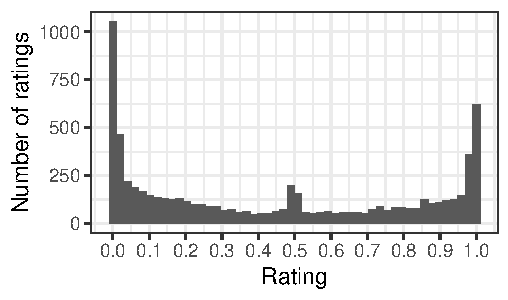
\includegraphics[width=\textwidth]{../../results/5-projectivity-no-fact/graphs/bunching}
\caption{Exp.~1a ratings.}
\label{fig:exp1araw}
\end{subfigure}
\begin{subfigure}{.33\textwidth}
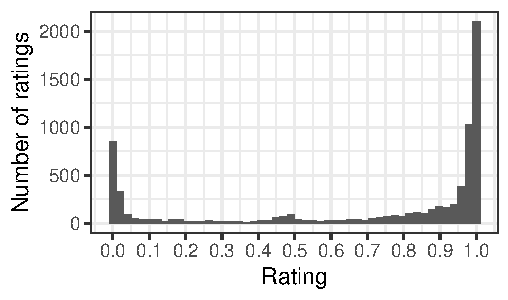
\includegraphics[width=\textwidth]{../../results/4-veridicality3/graphs/bunching}
\caption{Exp.~2a ratings.}
\label{fig:exp2araw}
\end{subfigure}
\begin{subfigure}{.33\textwidth}
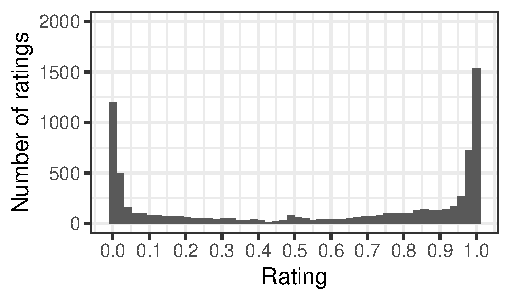
\includegraphics[width=\textwidth]{../../results/2-veridicality2/graphs/bunching}
\caption{Exp.~3a ratings.}
\label{fig:exp3araw}
\end{subfigure}
\caption{Histograms of raw slider ratings in Exps.~1a, 2a, and 3a.}
\label{fig:bunch}
\end{figure}

This `bunching' behavior, in turn, can lead to the violation of both of the above assumptions of linear regression. 
Intuitively, these assumptions are violated because conditions that elicit ratings closer to endpoints necessarily have a compressed variance; consequently, a condition's mean and its variance are not independent. Beta regression is useful here because it allows for modeling an arbitrarily distributed outcome variable in the $[$0,1$]$ interval. The Beta distribution is characterized by two parameters, one capturing the mean $\mu$ of the distribution and one capturing its precision $\phi$, a measure of dispersion. The greater the precision, the more concentrated the values are around the mean, that is, the lower the variance of the distribution.  We follow \citealt{smithson2006} in modeling $\mu$ and $\phi$ separately for each predictor. That is, we allow each predictor to affect both the mean and the precision of the outcome variable's distribution. 

\subsection{Coding choices and interpreting model output}\label{a-primer}

The outcome variable in Exps.~1a, 2a, and 3a (slider ratings) contained the values 0 and 1, which Beta regression is undefined for. We therefore applied a common transformation to ratings before the main analysis that rescales values $y$ to fall in the open unit interval (0,1)  \citep{smithson2006}. First, we apply $y' = (y-a)/(b-a)$, where $b$ is the highest possible slider rating and $a$ is the smallest possible slider rating. The range is then compressed to not include 0 and 1 by applying $y' = [y'(N-1) + 1/2]/N$, where $N$ is the total number of observations.

The mean parameter $\mu$ is modeled via a logit link function (default for Beta regression in \verb|brms|), though other links that squeeze $\mu$ into the $[$0,1$]$ interval are possible. The dispersion parameter $\phi$ is modeled via a log link, which ensures that values of $\phi$ are strictly positive, which is necessary because a variance cannot be negative. 

We allowed both $\mu$ and $\phi$ to vary as a function of predicate, with reference level set to main clause control in Exp.~1a, entailing control in Exp.~2a, and contradictory control in Exp.~3a. We also allowed random intercept adjustments to each parameter by participant and by item, where item was defined as a unique combination of a predicate and a complement clause. Four chains converged after 2000 iterations each (warmup = 1000, \(\hat{R}=1\) for all estimated parameters) with a target acceptance rate of .95 and a maximum treedepth of 15.

\subsection{Model outputs for Experiments 1, 2, and 3}\label{a-mo}

The three tables in this section show the model outputs for Exps.~1, 2, and 3, respectively: Table \ref{tab:exp1modelresults} for Exps.~1a and 1b, Table \ref{tab:exp2modelresults} for Exps.~2a and 2b, and Table \ref{tab:exp3modelresults} for Exps.~3a and 3b. Each table shows maximum a posteriori (MAP) model estimates for certainty ratings from the Beta regression model (left and middle column, mean $\mu$ and precision $\phi$) and the logistic regression model (right column, $\beta$)  with 95\% credible intervals.

\begin{table}
\caption{Maximum a posteriori (MAP) model estimates for certainty ratings from Exp.~1a (left and middle column, mean $\mu$ and precision $\phi$) and Exp.~1b (right column, $\beta$)  with 95\% credible intervals. Contrast of each predicate is with main clause control reference level. MAP estimates for which there is no evidence that they are different from 0 are italicized.}
\footnotesize
\begin{center}
\begin{tabular}{l c c c}
\toprule
& \multicolumn{2}{c}{Exp.~1a: Beta regression} & Exp.~1b: logistic regression \\
Predictor & Estimated $\mu$ & Estimated $\phi$ & Estimated $\beta$\\
\midrule
\multirow{2}{*}{Intercept} & $-1.88 $  & $1.16 $ & $-6.37 $       \\
& $[-1.98;\ -1.78]$ & $[1.02;\ 1.29]$  & $[-7.10;\ -5.72]$ \\
[.25em]
\multirow{2}{*}{acknowledge} & $2.62 $ & $-0.67 $  & $8.00 $        \\
& $[2.45;\ 2.80]$  & $[-0.86;\ -0.49]$ & $[7.31;\ 8.78]$   \\
[.25em]
\multirow{2}{*}{admit} & $2.45 $ & $-0.65 $  & $7.29 $        \\
& $[2.29;\ 2.61]$  & $[-0.83;\ -0.48]$ & $[6.60;\ 8.04]$   \\
[.25em]
\multirow{2}{*}{announce}  & $2.14 $ & $-0.74 $  & $6.70 $        \\
& $[1.98;\ 2.30]$  & $[-0.92;\ -0.57]$ & $[6.04;\ 7.45]$   \\
[.25em]
\multirow{2}{*}{be annoyed} & $3.56 $ & $-0.30 $  & $9.41 $        \\
& $[3.37;\ 3.75]$  & $[-0.51;\ -0.10]$ & $[8.64;\ 10.22]$  \\
[.25em]
\multirow{2}{*}{be right} & $0.52 $ & $-0.21 $  & $2.33 $        \\
& $[0.36;\ 0.68]$  & $[-0.40;\ -0.01]$ & $[1.50;\ 3.21]$   \\
[.25em]
\multirow{2}{*}{confess} & $2.29 $ & $-0.71 $  & $6.75 $        \\
& $[2.13;\ 2.45]$  & $[-0.88;\ -0.54]$ & $[6.07;\ 7.50]$   \\
[.25em]
\multirow{2}{*}{confirm} & $1.31 $ & $-0.46 $  & $4.27 $        \\
& $[1.15;\ 1.46]$  & $[-0.64;\ -0.28]$ & $[3.60;\ 5.01]$   \\
[.25em]
\multirow{2}{*}{demonstrate} & $1.78 $ & $-0.59 $  & $5.31 $        \\
& $[1.63;\ 1.93]$  & $[-0.76;\ -0.41]$ & $[4.64;\ 6.06]$   \\
[.25em]
\multirow{2}{*}{discover}  & $2.90 $ & $-0.67 $  & $8.46 $        \\
& $[2.72;\ 3.07]$  & $[-0.85;\ -0.48]$ & $[7.75;\ 9.25]$   \\
[.25em]
\multirow{2}{*}{establish} & $1.42 $ & $-0.55 $  & $4.51 $        \\
& $[1.26;\ 1.58]$  & $[-0.73;\ -0.38]$ & $[3.83;\ 5.26]$   \\
[.25em]
\multirow{2}{*}{hear}  & $2.71 $ & $-0.79 $  & $8.22 $        \\
& $[2.53;\ 2.88]$  & $[-0.98;\ -0.61]$ & $[7.50;\ 9.01]$   \\
[.25em]
\multirow{2}{*}{inform}  & $3.00 $ & $-0.60 $  & $9.13 $        \\
& $[2.82;\ 3.18]$  & $[-0.79;\ -0.41]$ & $[8.38;\ 9.94]$   \\
[.25em]
\multirow{2}{*}{know}  & $3.37 $ & $-0.49 $  & $9.72 $        \\
& $[3.18;\ 3.56]$  & $[-0.70;\ -0.29]$ & $[8.94;\ 10.57]$  \\
[.25em]
\multirow{2}{*}{pretend} & $0.32 $ & $-0.19 $  & $3.22 $        \\
& $[0.15;\ 0.49]$  & $[-0.38;\ -0.00]$ & $[2.50;\ 4.03]$   \\
[.25em]
\multirow{2}{*}{prove} & $1.16 $ & $-0.21 $  & $3.92 $        \\
& $[1.01;\ 1.31]$  & $[-0.40;\ -0.03]$ & $[3.21;\ 4.67]$   \\
[.25em]
\multirow{2}{*}{reveal}  & $2.59 $ & $-0.72 $  & $7.41 $        \\
& $[2.42;\ 2.76]$  & $[-0.90;\ -0.55]$ & $[6.72;\ 8.16]$   \\
[.25em]
\multirow{2}{*}{say} & $0.78 $ & \emph{-0.12}  & $3.10 $        \\
& $[0.63;\ 0.93]$  & $[-0.30;\ 0.06]$ & $[2.35;\ 3.93]$   \\
[.25em]
\multirow{2}{*}{see} & $3.01 $ & $-0.70 $  & $8.74 $        \\
& $[2.83;\ 3.19]$  & $[-0.90;\ -0.51]$ & $[8.03;\ 9.55]$   \\
[.25em]
\multirow{2}{*}{suggest} & $0.79 $ & \emph{-0.17}  & $3.22 $        \\
& $[0.63;\ 0.94]$  & $[-0.36;\ 0.02]$ & $[2.49;\ 3.99]$   \\
[.25em]
\multirow{2}{*}{think} & $0.62 $ & \emph{0.01} & $2.54 $        \\
& $[0.47;\ 0.78]$  & $[-0.17;\ 0.20]$ & $[1.75;\ 3.40]$   \\
\bottomrule
\end{tabular}
\label{tab:exp1modelresults}
\end{center}
\end{table}

\normalsize


\begin{table}
\caption{Maximum a posteriori (MAP) model estimates for inference ratings from Exp.~2a (left and middle column, mean $\mu$ and precision $\phi$) and Exp.~2b (right column, $\beta$)  with 95\% credible intervals. Contrast of each predicate is with entailing control reference level. MAP estimates for which there is no evidence that they are different from 0 are italicized. Predicates are marked for which there is no evidence that they differ from  entailing controls (bold: no difference on either categorical or continuous measure; italics: no difference on at least one measure).}
\footnotesize
\begin{center}
\begin{tabular}{l c c c}
\toprule
& \multicolumn{2}{c}{Exp.~2a: Beta regression} & Exp.~2b: logistic regression \\
Predictor & Estimated $\mu$ & Estimated $\phi$ & Estimated $\beta$\\
\midrule
\multirow{2}{*}{Intercept}            & $3.00$        & $2.24$        & $6.20$          \\
                        & $[2.87;\ 3.15]$   & $[2.05;\ 2.42]$   & $[5.52;\ 6.98]$     \\
\multirow{2}{*}{acknowledge}      & $-0.74$       & $-0.64$       & $-1.58$         \\
                        & $[-0.94;\ -0.54]$ & $[-0.89;\ -0.39]$ & $[-2.47;\ -0.70]$   \\
\multirow{2}{*}{admit}            & $-0.67$       & $-0.52$       & $-1.83$         \\
                        & $[-0.87;\ -0.48]$ & $[-0.77;\ -0.27]$ & $[-2.72;\ -0.97]$   \\
\multirow{2}{*}{announce}         & $-1.51$       & $-1.35$       & $-4.39$         \\
                        & $[-1.71;\ -1.31]$ & $[-1.59;\ -1.10]$ & $[-5.17;\ -3.68]$   \\
\multirow{2}{*}{be annoyed}      & $-0.55$       & $-0.50$       & $-1.36$         \\
                        & $[-0.76;\ -0.35]$ & $[-0.75;\ -0.23]$ & $[-2.31;\ -0.46]$   \\
\multirow{2}{*}{\textbf{be right}}        & \emph{-0.03}           & \emph{0.09}            & \emph{0.36}              \\
                        & $[-0.22;\ 0.16]$  & $[-0.16;\ 0.34]$  & $[-0.93;\ 1.89]$    \\
\multirow{2}{*}{confess}          & $-0.85$       & $-0.64$       & $-2.79$         \\
                        & $[-1.05;\ -0.66]$ & $[-0.90;\ -0.38]$ & $[-3.60;\ -2.04]$   \\
\multirow{2}{*}{\emph{confirm}}          & $-0.22$       & \emph{-0.00}           & \emph{-0.85}             \\
                        & $[-0.41;\ -0.03]$ & $[-0.26;\ 0.26]$  & $[-1.84;\ 0.14]$    \\
\multirow{2}{*}{demonstrate}      & $-1.23$       & $-1.18$       & $-3.35$         \\
                        & $[-1.44;\ -1.02]$ & $[-1.44;\ -0.93]$ & $[-4.15;\ -2.63]$   \\
\multirow{2}{*}{\emph{discover}}         & $-0.27$       & \emph{-0.10}           & \emph{-0.50}             \\
                        & $[-0.46;\ -0.08]$ & $[-0.35;\ 0.14]$  & $[-1.57;\ 0.64]$    \\
\multirow{2}{*}{establish}        & $-0.78$       & $-0.68$       & $-1.92$         \\
                        & $[-0.98;\ -0.58]$ & $[-0.92;\ -0.42]$ & $[-2.76;\ -1.12]$   \\
\multirow{2}{*}{hear}             & $-2.92$       & $-2.05$       & $-7.57$         \\
                        & $[-3.12;\ -2.72]$ & $[-2.27;\ -1.83]$ & $[-8.41;\ -6.84]$   \\
\multirow{2}{*}{inform}           & $-1.37$       & $-1.29$       & $-3.93$         \\
                        & $[-1.57;\ -1.16]$ & $[-1.54;\ -1.05]$ & $[-4.71;\ -3.22]$   \\
\multirow{2}{*}{know}             & $-0.40$       & $-0.28$       & $-0.27$             \\
                        & $[-0.60;\ -0.21]$ & $[-0.54;\ -0.03]$ & $[-1.39;\ 0.96]$    \\
\multirow{2}{*}{nonMent.C}        & $-6.22$       & $-0.27$       & $-11.92$        \\
                        & $[-6.42;\ -6.02]$ & $[-0.52;\ -0.04]$ & $[-12.94;\ -11.01]$ \\
\multirow{2}{*}{pretend}          & $-4.47$       & $-2.13$       & $-10.78$        \\
                        & $[-4.72;\ -4.24]$ & $[-2.38;\ -1.87]$ & $[-11.83;\ -9.85]$  \\
\multirow{2}{*}{\textbf{prove}}            & \emph{-0.08}           & \emph{-0.13}           & \emph{0.92}              \\
                        & $[-0.29;\ 0.14]$  & $[-0.40;\ 0.14]$  & $[-0.57;\ 2.91]$    \\
\multirow{2}{*}{reveal}           & $-0.80$       & $-0.67$       & $-2.37$         \\
                        & $[-1.00;\ -0.60]$ & $[-0.92;\ -0.41]$ & $[-3.21;\ -1.54]$   \\
\multirow{2}{*}{say}              & $-2.20$       & $-1.92$       & $-5.79$         \\
                        & $[-2.41;\ -2.00]$ & $[-2.15;\ -1.69]$ & $[-6.59;\ -5.09]$   \\
\multirow{2}{*}{\emph{see}}              & $-0.23$       & \emph{-0.16}           & \emph{-0.49}             \\
                        & $[-0.43;\ -0.02]$ & $[-0.41;\ 0.09]$  & $[-1.51;\ 0.62]$    \\
\multirow{2}{*}{suggest}          & $-3.47$       & $-1.90$       & $-8.75$         \\
                        & $[-3.67;\ -3.27]$ & $[-2.12;\ -1.67]$ & $[-9.62;\ -7.95]$   \\
\multirow{2}{*}{think}            & $-3.64$       & $-1.85$       & $-9.71$         \\
                        & $[-3.84;\ -3.44]$ & $[-2.08;\ -1.62]$ & $[-10.65;\ -8.87]$  \\
\bottomrule
\end{tabular}
\label{tab:exp2modelresults}
\end{center}
\end{table}

\normalsize

\begin{table}
\caption{Maximum a posteriori (MAP) model estimates for contradictoriness ratings from Exp.~3a (left and middle column, mean $\mu$ and precision $\phi$) and Exp.~3b (right column, $\beta$)  with 95\% credible intervals. Contrast of each predicate is with contradictory control reference level. MAP estimates for which there is no evidence that they are different from 0 are italicized.}
\footnotesize
\begin{center}
\begin{tabular}{l c c c}
\toprule
& \multicolumn{2}{c}{Exp.~3a: Beta regression} & Exp.~3b: logistic regression \\
Predictor & Estimated $\mu$ & Estimated $\phi$ & Estimated $\beta$\\
\midrule
\multirow{2}{*}{Intercept}             & $2.74$        & $1.46$        & $6.17$          \\
                         & $[2.54;\ 2.93]$   & $[1.23;\ 1.66]$   & $[5.55;\ 6.88]$     \\
\multirow{2}{*}{acknowledge}       & $-2.15$       & $-1.04$       & $-4.89$         \\
                         & $[-2.39;\ -1.90]$ & $[-1.29;\ -0.79]$ & $[-5.65;\ -4.21]$   \\
\multirow{2}{*}{admit}             & $-2.03$       & $-1.05$       & $-4.86$         \\
                         & $[-2.26;\ -1.77]$ & $[-1.30;\ -0.78]$ & $[-5.59;\ -4.19]$   \\
\multirow{2}{*}{announce}          & $-2.90$       & $-1.56$       & $-6.46$         \\
                         & $[-3.14;\ -2.64]$ & $[-1.80;\ -1.32]$ & $[-7.20;\ -5.80]$   \\
\multirow{2}{*}{be annoyed}       & $-2.24$       & $-1.28$       & $-5.18$         \\
                         & $[-2.47;\ -1.98]$ & $[-1.53;\ -1.03]$ & $[-5.91;\ -4.51]$   \\
\multirow{2}{*}{be right}         & $-0.40$       & \emph{-0.18}           & $-1.90$         \\
                         & $[-0.67;\ -0.12]$ & $[-0.48;\ 0.12]$  & $[-2.70;\ -1.12]$   \\
\multirow{2}{*}{confess}           & $-2.15$       & $-1.12$       & $-4.85$         \\
                         & $[-2.39;\ -1.89]$ & $[-1.37;\ -0.86]$ & $[-5.59;\ -4.18]$   \\
\multirow{2}{*}{confirm}           & $-1.74$       & $-0.99$       & $-4.25$         \\
                         & $[-1.99;\ -1.48]$ & $[-1.24;\ -0.73]$ & $[-4.99;\ -3.57]$   \\
\multirow{2}{*}{demonstrate}       & $-1.94$       & $-1.05$       & $-4.53$         \\
                         & $[-2.18;\ -1.69]$ & $[-1.30;\ -0.79]$ & $[-5.25;\ -3.84]$   \\
\multirow{2}{*}{discover}          & $-1.63$       & $-1.02$       & $-3.30$         \\
                         & $[-1.90;\ -1.38]$ & $[-1.27;\ -0.75]$ & $[-4.06;\ -2.61]$   \\
\multirow{2}{*}{establish}         & $-1.94$       & $-1.00$       & $-4.29$         \\
                         & $[-2.19;\ -1.70]$ & $[-1.27;\ -0.75]$ & $[-5.06;\ -3.62]$   \\
\multirow{2}{*}{hear}              & $-3.72$       & $-1.29$       & $-8.98$         \\
                         & $[-3.97;\ -3.45]$ & $[-1.54;\ -1.01]$ & $[-9.79;\ -8.27]$   \\
\multirow{2}{*}{inform}            & $-2.78$       & $-1.51$       & $-6.46$         \\
                         & $[-3.03;\ -2.52]$ & $[-1.75;\ -1.25]$ & $[-7.20;\ -5.81]$   \\
\multirow{2}{*}{know}              & $-1.37$       & $-0.90$       & $-3.64$         \\
                         & $[-1.63;\ -1.11]$ & $[-1.17;\ -0.64]$ & $[-4.39;\ -2.95]$   \\
\multirow{2}{*}{non-contra.~control}      & $-5.26$       & \emph{-0.24}           & $-11.51$        \\
                         & $[-5.54;\ -4.98]$ & $[-0.51;\ 0.04]$  & $[-12.43;\ -10.71]$ \\
\multirow{2}{*}{pretend}           & $-3.72$       & $-1.35$       & $-8.97$         \\
                         & $[-3.98;\ -3.46]$ & $[-1.61;\ -1.10]$ & $[-9.78;\ -8.26]$   \\
\multirow{2}{*}{prove}             & $-1.18$       & $-0.71$       & $-3.36$         \\
                         & $[-1.44;\ -0.92]$ & $[-0.98;\ -0.45]$ & $[-4.10;\ -2.65]$   \\
\multirow{2}{*}{reveal}            & $-2.27$       & $-1.24$       & $-4.99$         \\
                         & $[-2.52;\ -2.02]$ & $[-1.50;\ -0.98]$ & $[-5.73;\ -4.32]$   \\
\multirow{2}{*}{say}               & $-3.17$       & $-1.51$       & $-7.11$         \\
                         & $[-3.42;\ -2.91]$ & $[-1.75;\ -1.25]$ & $[-7.87;\ -6.42]$   \\
\multirow{2}{*}{see}               & $-1.43$       & $-0.82$       & $-3.48$         \\
                         & $[-1.68;\ -1.18]$ & $[-1.08;\ -0.56]$ & $[-4.21;\ -2.78]$   \\
\multirow{2}{*}{suggest}           & $-3.58$       & $-1.17$       & $-8.92$         \\
                         & $[-3.83;\ -3.31]$ & $[-1.43;\ -0.92]$ & $[-9.71;\ -8.21]$   \\
\multirow{2}{*}{think}             & $-3.93$       & $-1.20$       & $-9.81$         \\
                         & $[-4.19;\ -3.66]$ & $[-1.47;\ -0.94]$ & $[-10.67;\ -9.06]$  \\
\bottomrule
\end{tabular}
\label{tab:exp3modelresults}
\end{center}
\end{table}

\normalsize


\section{Comparisons of gradient and categorical ratings}\label{a-comparison}

The Spearman rank correlation coefficient, a value between -1 and 1, is a nonparametric measure of rank correlation: the higher the coefficient, the more the relation between the the two variables can be described using a monotonic function; if the coefficient is positive, the value of one variable tends to increase with an increase in the other. For instance, in the case of our Exps.~1, a coefficient of 1 would mean that there is a perfectly monotone increasing relation between the mean certainty ratings of the predicates in Exp.~1a and Exp.~1b: for any two predicates $p_1$ and $p_2$, if $p_1$ ranks below $p_2$ in Exp.~1a (that is, the mean certainty rating of $p_1$ is lower than that of $p_2$), then that ranking is preserved in Exp.~1b.

The three panels of Figure \ref{f-comparison} visualize the strong correlation between by-predicate mean ratings in Exps.~1a, 2a, and 3a and by-predicate proportion of `yes' responses in Exps.~1b, 2b, and 3b, respectively.

\begin{figure}[h!]
\centering
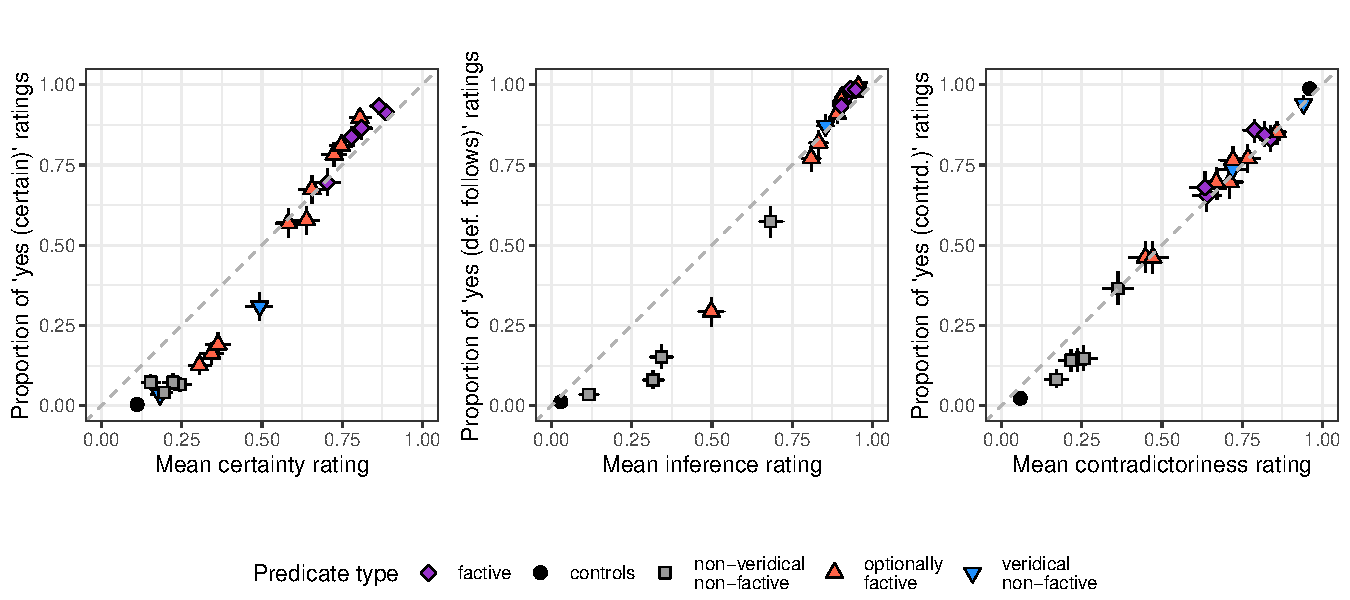
\includegraphics[width=.75\paperwidth]{../../results/compare-diagnostics-and-response-tasks/graphs/joint-comparison-plot}
   
\caption{By-predicate proportion of `yes' responses in two-alternative forced choice task against mean slider ratings in Exps.~1 (left, $r=.98$), Exps.~2 (middle, $r=.99$), and Exps.~3 (right, $r=.99$). Error bars indicate 95\% bootstrapped confidence intervals.}
\label{f-comparison}
\end{figure}

\section{Mixture models applied to data from Exp.~1a}\label{a-gaussian}

Figure \ref{fig:mixtures-exp1a} plots the density of certainty ratings for the 20 predicates from Exp.~1a with the number of Gaussian components overlaid.

\begin{sidewaysfigure}[h!]
\centering

\begin{subfigure}{.19\textheight}
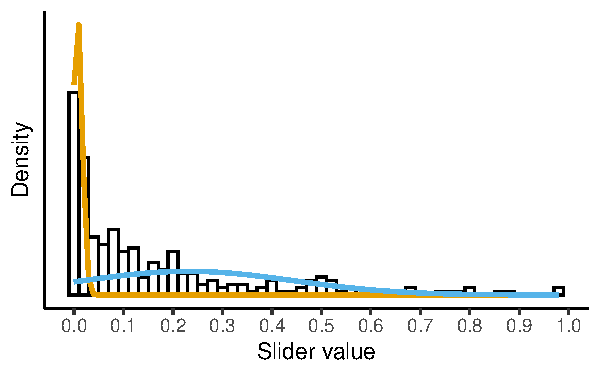
\includegraphics[width=\textwidth]{../../results/5-projectivity-no-fact/graphs/mixtures/predicates/pretend-gaussian}
\caption{{\em pretend}, 2 components.}
\label{fig:1comp}
\end{subfigure} \begin{subfigure}{.19\textheight}
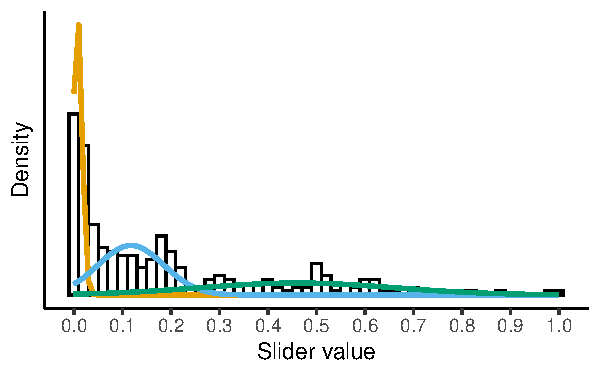
\includegraphics[width=\textwidth]{../../results/5-projectivity-no-fact/graphs/mixtures/predicates/be-right-gaussian}
\caption{{\em be right}, 3 components.}
\label{fig:1comp}
\end{subfigure} 
\begin{subfigure}{.19\textheight}
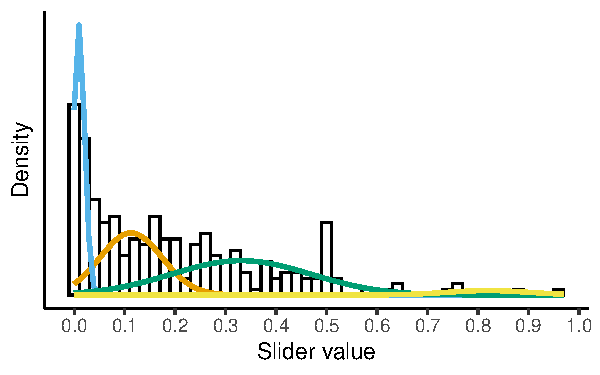
\includegraphics[width=\textwidth]{../../results/5-projectivity-no-fact/graphs/mixtures/predicates/think-gaussian}
\caption{{\em think}, 4 components.}
\label{fig:1comp}
\end{subfigure}
\begin{subfigure}{.19\textheight}
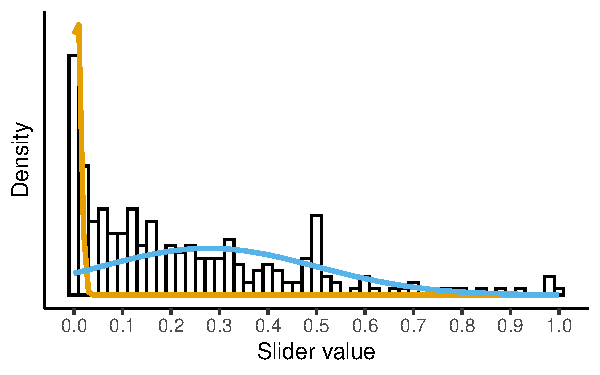
\includegraphics[width=\textwidth]{../../results/5-projectivity-no-fact/graphs/mixtures/predicates/suggest-gaussian}
\caption{{\em suggest}, 2 components.}
\label{fig:1comp}
\end{subfigure}
\begin{subfigure}{.19\textheight}
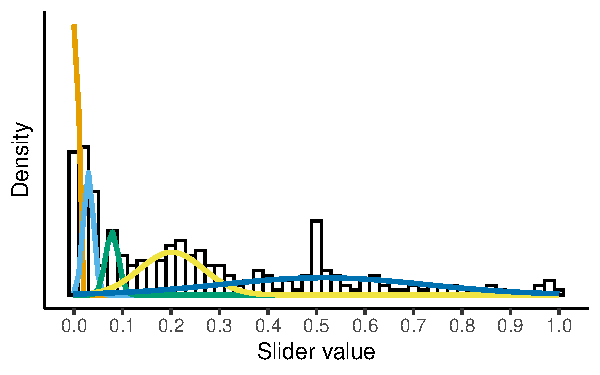
\includegraphics[width=\textwidth]{../../results/5-projectivity-no-fact/graphs/mixtures/predicates/say-gaussian}
\caption{{\em say}, 5 components.}
\label{fig:1comp}
\end{subfigure}

\begin{subfigure}{.19\textheight}
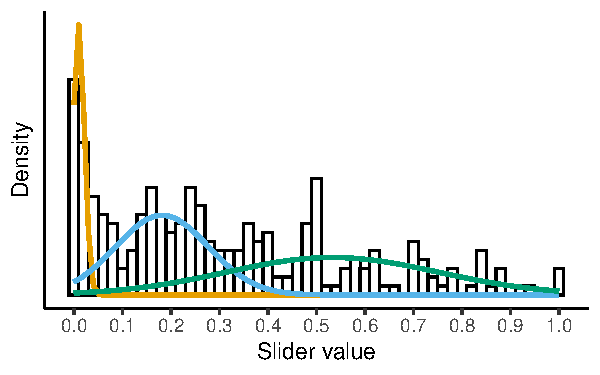
\includegraphics[width=\textwidth]{../../results/5-projectivity-no-fact/graphs/mixtures/predicates/prove-gaussian}
\caption{{\em prove}, 3 components.}
\label{fig:1comp}
\end{subfigure}
\begin{subfigure}{.19\textheight}
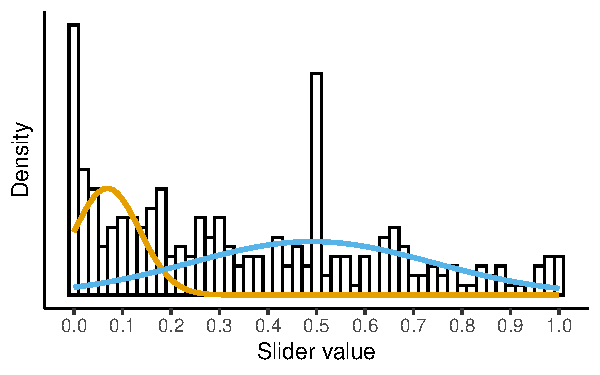
\includegraphics[width=\textwidth]{../../results/5-projectivity-no-fact/graphs/mixtures/predicates/confirm-gaussian}
\caption{{\em confirm}, 2 components.}
\label{fig:1comp}
\end{subfigure}
\begin{subfigure}{.19\textheight}
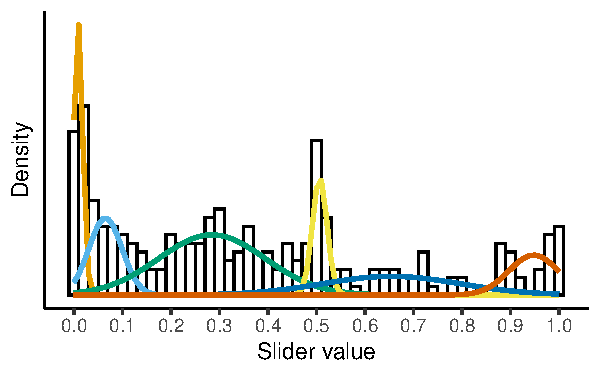
\includegraphics[width=\textwidth]{../../results/5-projectivity-no-fact/graphs/mixtures/predicates/establish-gaussian}
\caption{{\em establish}, 6 components.}
\label{fig:1comp}
\end{subfigure}
\begin{subfigure}{.19\textheight}
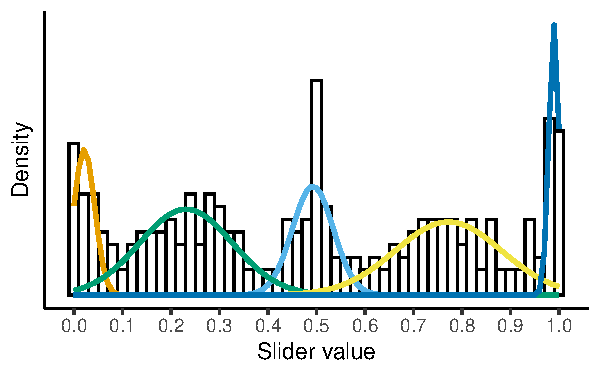
\includegraphics[width=\textwidth]{../../results/5-projectivity-no-fact/graphs/mixtures/predicates/demonstrate-gaussian}
\caption{{\em demonstrate}, 5 components.}
\label{fig:1comp}
\end{subfigure}
\begin{subfigure}{.19\textheight}
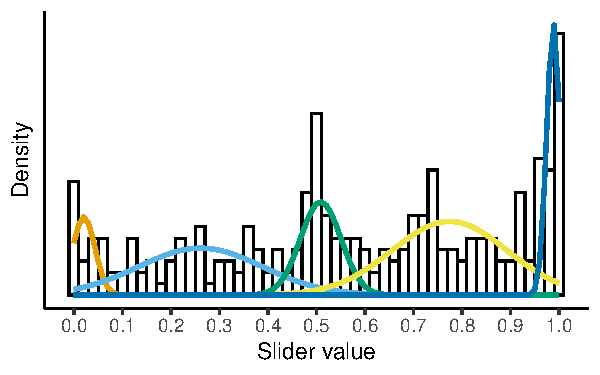
\includegraphics[width=\textwidth]{../../results/5-projectivity-no-fact/graphs/mixtures/predicates/announce-gaussian}
\caption{{\em announce}, 5 components.}
\label{fig:1comp}
\end{subfigure}

\begin{subfigure}{.19\textheight}
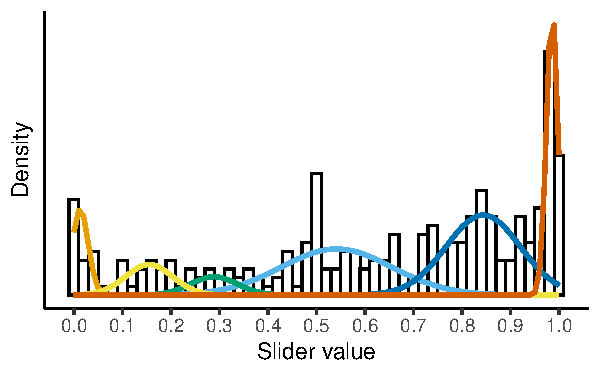
\includegraphics[width=\textwidth]{../../results/5-projectivity-no-fact/graphs/mixtures/predicates/confess-gaussian}
\caption{{\em confess}, 6 components.}
\label{fig:1comp}
\end{subfigure}
\begin{subfigure}{.19\textheight}
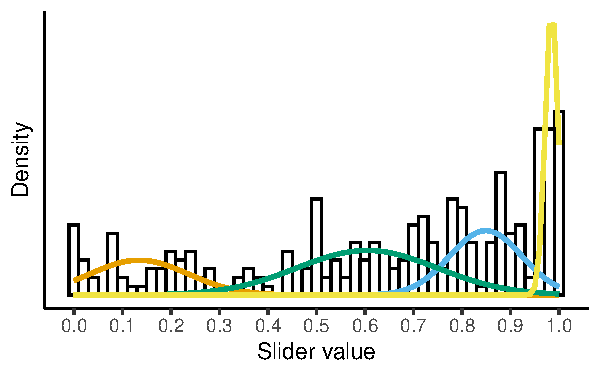
\includegraphics[width=\textwidth]{../../results/5-projectivity-no-fact/graphs/mixtures/predicates/admit-gaussian}
\caption{{\em admit}, 4 components.}
\label{fig:1comp}
\end{subfigure}
\begin{subfigure}{.19\textheight}
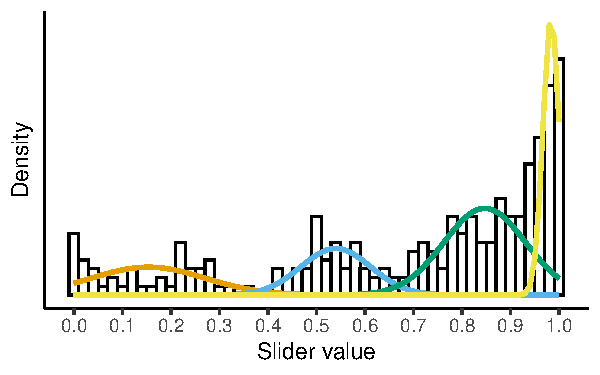
\includegraphics[width=\textwidth]{../../results/5-projectivity-no-fact/graphs/mixtures/predicates/reveal-gaussian}
\caption{{\em reveal}, 4 components.}
\label{fig:1comp}
\end{subfigure}
\begin{subfigure}{.19\textheight}
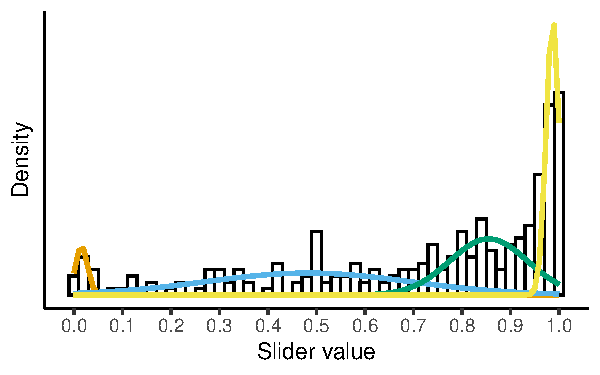
\includegraphics[width=\textwidth]{../../results/5-projectivity-no-fact/graphs/mixtures/predicates/acknowledge-gaussian}
\caption{{\em acknowledge}, 4 components.}
\label{fig:1comp}
\end{subfigure}
\begin{subfigure}{.19\textheight}
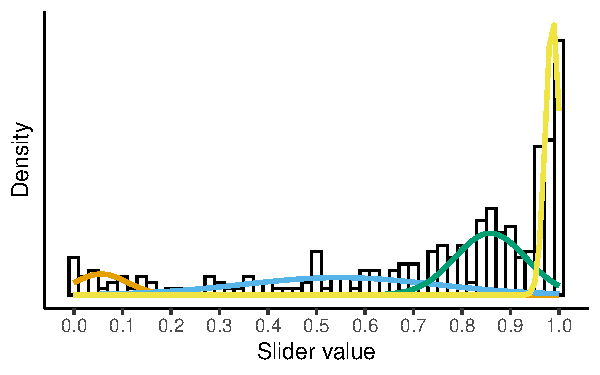
\includegraphics[width=\textwidth]{../../results/5-projectivity-no-fact/graphs/mixtures/predicates/hear-gaussian}
\caption{{\em hear}, 4 components.}
\label{fig:1comp}
\end{subfigure}

\begin{subfigure}{.19\textheight}
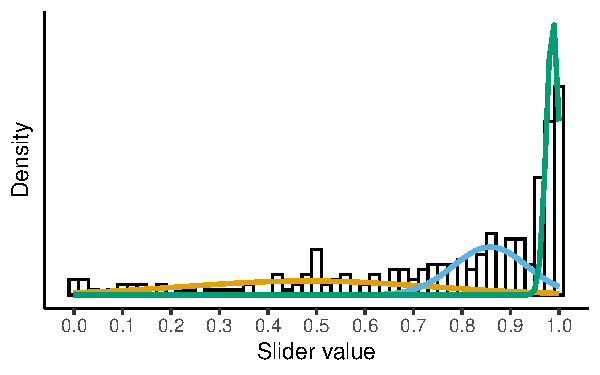
\includegraphics[width=\textwidth]{../../results/5-projectivity-no-fact/graphs/mixtures/predicates/discover-gaussian}
\caption{{\em admit}, 4 components.}
\label{fig:1comp}
\end{subfigure}
\begin{subfigure}{.19\textheight}
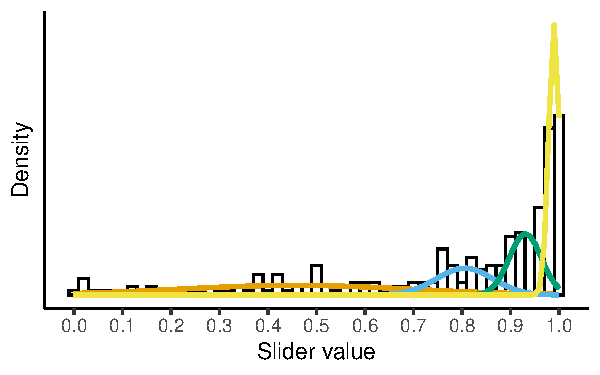
\includegraphics[width=\textwidth]{../../results/5-projectivity-no-fact/graphs/mixtures/predicates/inform-gaussian}
\caption{{\em inform}, 4 components.}
\label{fig:1comp}
\end{subfigure}
\begin{subfigure}{.19\textheight}
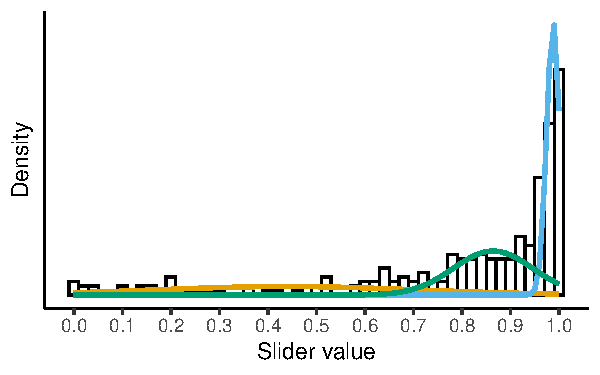
\includegraphics[width=\textwidth]{../../results/5-projectivity-no-fact/graphs/mixtures/predicates/see-gaussian}
\caption{{\em see}, 3 components.}
\label{fig:1comp}
\end{subfigure}
\begin{subfigure}{.19\textheight}
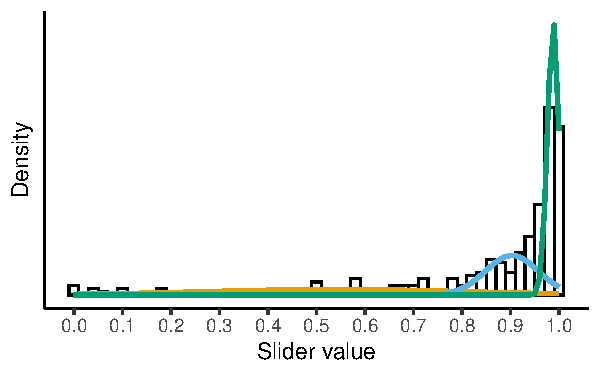
\includegraphics[width=\textwidth]{../../results/5-projectivity-no-fact/graphs/mixtures/predicates/know-gaussian}
\caption{{\em know}, 3 components.}
\label{fig:1comp}
\end{subfigure}
\begin{subfigure}{.19\textheight}
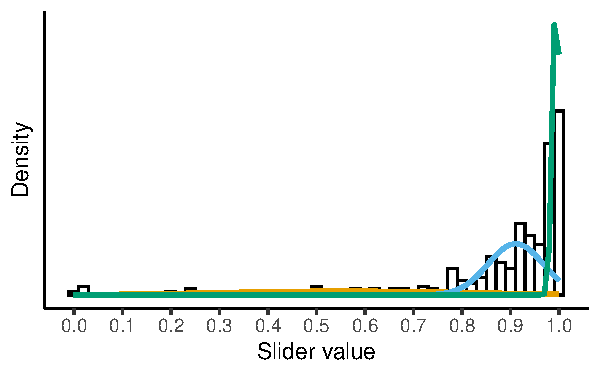
\includegraphics[width=\textwidth]{../../results/5-projectivity-no-fact/graphs/mixtures/predicates/be-annoyed-gaussian}
\caption{{\em be annoyed}, 3 components.}
\label{fig:1comp}
\end{subfigure}

\caption{Histograms of certainty ratings from Exp.~1a with overlaid optimal number of Gaussian components.}
\label{fig:mixtures-exp1a}
\end{sidewaysfigure}

%\bibliographystyle{../cslipubs-natbib}
\bibliography{../../bibliography}

\end{document}

